\documentclass[a4paper,twoside,kulak]{kulakreport} %options: kul or kulak (default)

\usepackage[utf8]{inputenc}
\usepackage[dutch]{babel}
\usepackage{eurosym}
\usepackage[utf8]{inputenc}
\usepackage[dutch]{babel}
\usepackage{siunitx}
\usepackage{graphicx}
\usepackage{flafter}
\usepackage{pdfpages}
\usepackage{caption}
\usepackage{subcaption}

\faculty{Wetenschap \& Technologie Kulak}
\group{Ingenieurswetenschappen}
\title{How to make \textit{an automated microplate dispenser}}
\subtitle{Een zoektocht naar precisie, snelheid en }
\author{Team ELISA}
\institute{Matthias Derez, Maxime Dujardin, Korneel Verkens, Seppe Vilain}
\date{Academiejaar 2019 -- 2020}
\address{
   KU Leuven Kulak           \\
   Wetenschap \& Technologie \\
   Etienne Sabbelaan 53, 8500 Kortrijk                \\
   \href{mailto:\theemailaddress}{\texttt{\theemailaddress}}
   }

\begin{document} % hier begint de eigenlijke inhoud van het document

\titlepage

\tableofcontents

\chapter*{Inleiding}
Inleidende tekst.

\chapter{Klantenvereisten}
De klant wil een geautomatiseerde \textit{dispenser}. De \textit{dispenser} moet in staat zijn om volledig autonoom een \textit{microwell}-plaat te vullen met de te onderzoeken substantie. Dit alles moet kunnen zonder dat er fouten gemaakt worden: dit betekent dat in elke \textit{microwell} exact evenveel substantie moet zitten en dat er niet naast de \textit{microwells} mag gemorst worden. Bovendien moet dit alles kunnen in een tijd die aanzienlijk korter is dan wanneer men deze \textit{microwell}-plaat handmatig zou vullen. Vooral dit laatse is belangrijk, aangezien het vullen van de platen een zeer arbeidsintensief en tijdrovend aspect is bij de ELISA-test. Het apparaat moet eenvoudig te bedienen zijn en de pipetpunten die de substantie in de \textit{wells} spuiten, moeten vervangbaar zijn. Er is een budget van \EUR{50} tot \EUR{75} voorzien. 

\chapter{Ontwerpspecificaties}
De te onderzoeken substantie bevindt zich in een recipiënt van waaruit het kan worden opgezogen. De \textit{microwell}-plaat is 27.76 mm breed, 85.48 mm lang en 14.4 mm hoog. Er zitten 96 \textit{microwells} in, met een bovendiameter van 6.96 mm en een benedendiameter van 6.58 mm (zie Figuur \ref{fig: afmetingenMicrowellplaat}). Het werkvolume van elke \textit{well} is tussen 25 $\mu l$ en 340 $\mu l$. De middelpunten van de \textit{wells} bevinden zich op 9 mm van elkaar. De middelpunten van de pipetpunten moeten dus op 9 mm van elkaar zitten en moeten verwijderbaar zijn. De machine moet elke \textit{well} kunnen vullen met een hoeveelheid van 100 $\mu l$ of 200 $\mu l$ van de te onderzoeken substantie. Om de vloeistof niet te morsen naast de \textit{wells}, moeten de pipetpunten telkens exact boven het middelpunt van de \textit{well} de vloeistof lossen. Om het apparaat gebruikvriendelijk te maken, moet een grafische interface voorzien worden, zodat de machine in enkele tellen kan opgestart worden.

\begin{figure}[h]
	\centering
	\includegraphics[width=0.5\textwidth]{AfmetingenMicrowell.png}
	\caption{Afmetingen \textit{microwell}-plaat}
	\label{fig: afmetingenMicrowellplaat}
	
\end{figure} 


\chapter{Ontwerpen} 
\section{Mogelijke \textit{concepts}}
\subsection{Concept 1}
Een eerste concept is gebaseerd op het principe van een handmatige \textit{dispenser} die ter beschikking werd gesteld. In Figuur \ref{fig: schets concept 1} staat een schets van het \textit{concept}. De \textit{wells} worden in dit concept gevuld door 96 cilinders. De cilinders zijn vastgemaakt aan een plaat in 12 rijen van 8. De afstand tussen de middelpunten van 2 cilinders is telkens 9 mm. De cilinders zelf bewegen niet. In elke cilinder zit een zuiger die op en neer kan bewegen. De koppen van de cilinders zijn vastgemaakt op een plaat die op en neer kan bewegen (zie Figuur \ref{fig: foto concept 1 zuiger}) m.b.v. een motor die boven het geheel van de twee platen is bevestigd. Het geheel van de platen met de zuigers en cilinders kan op en neer bewegen om de vloeistof in de cilinders op te zuigen. De \textit{microwell}-plaat is bevestigd aan een aandrijfriem met een motor zodat de plaat naar links en rechts kan bewegen. Dit laat het mechanisme toe om telkens de cilinders opnieuw te vullen en een gevulde \textit{microwell}-plaat te vervangen door een lege.  

\begin{figure}[h]
	\centering
	\includegraphics[width=0.8\textwidth]{fotoConcept1.jpg}
	\caption{Schets \textit{concept} 1}
	\label{fig: schets concept 1}
	
\end{figure} 

\begin{figure}
	\centering
	\begin{subfigure}{.5\textwidth}
		\centering
		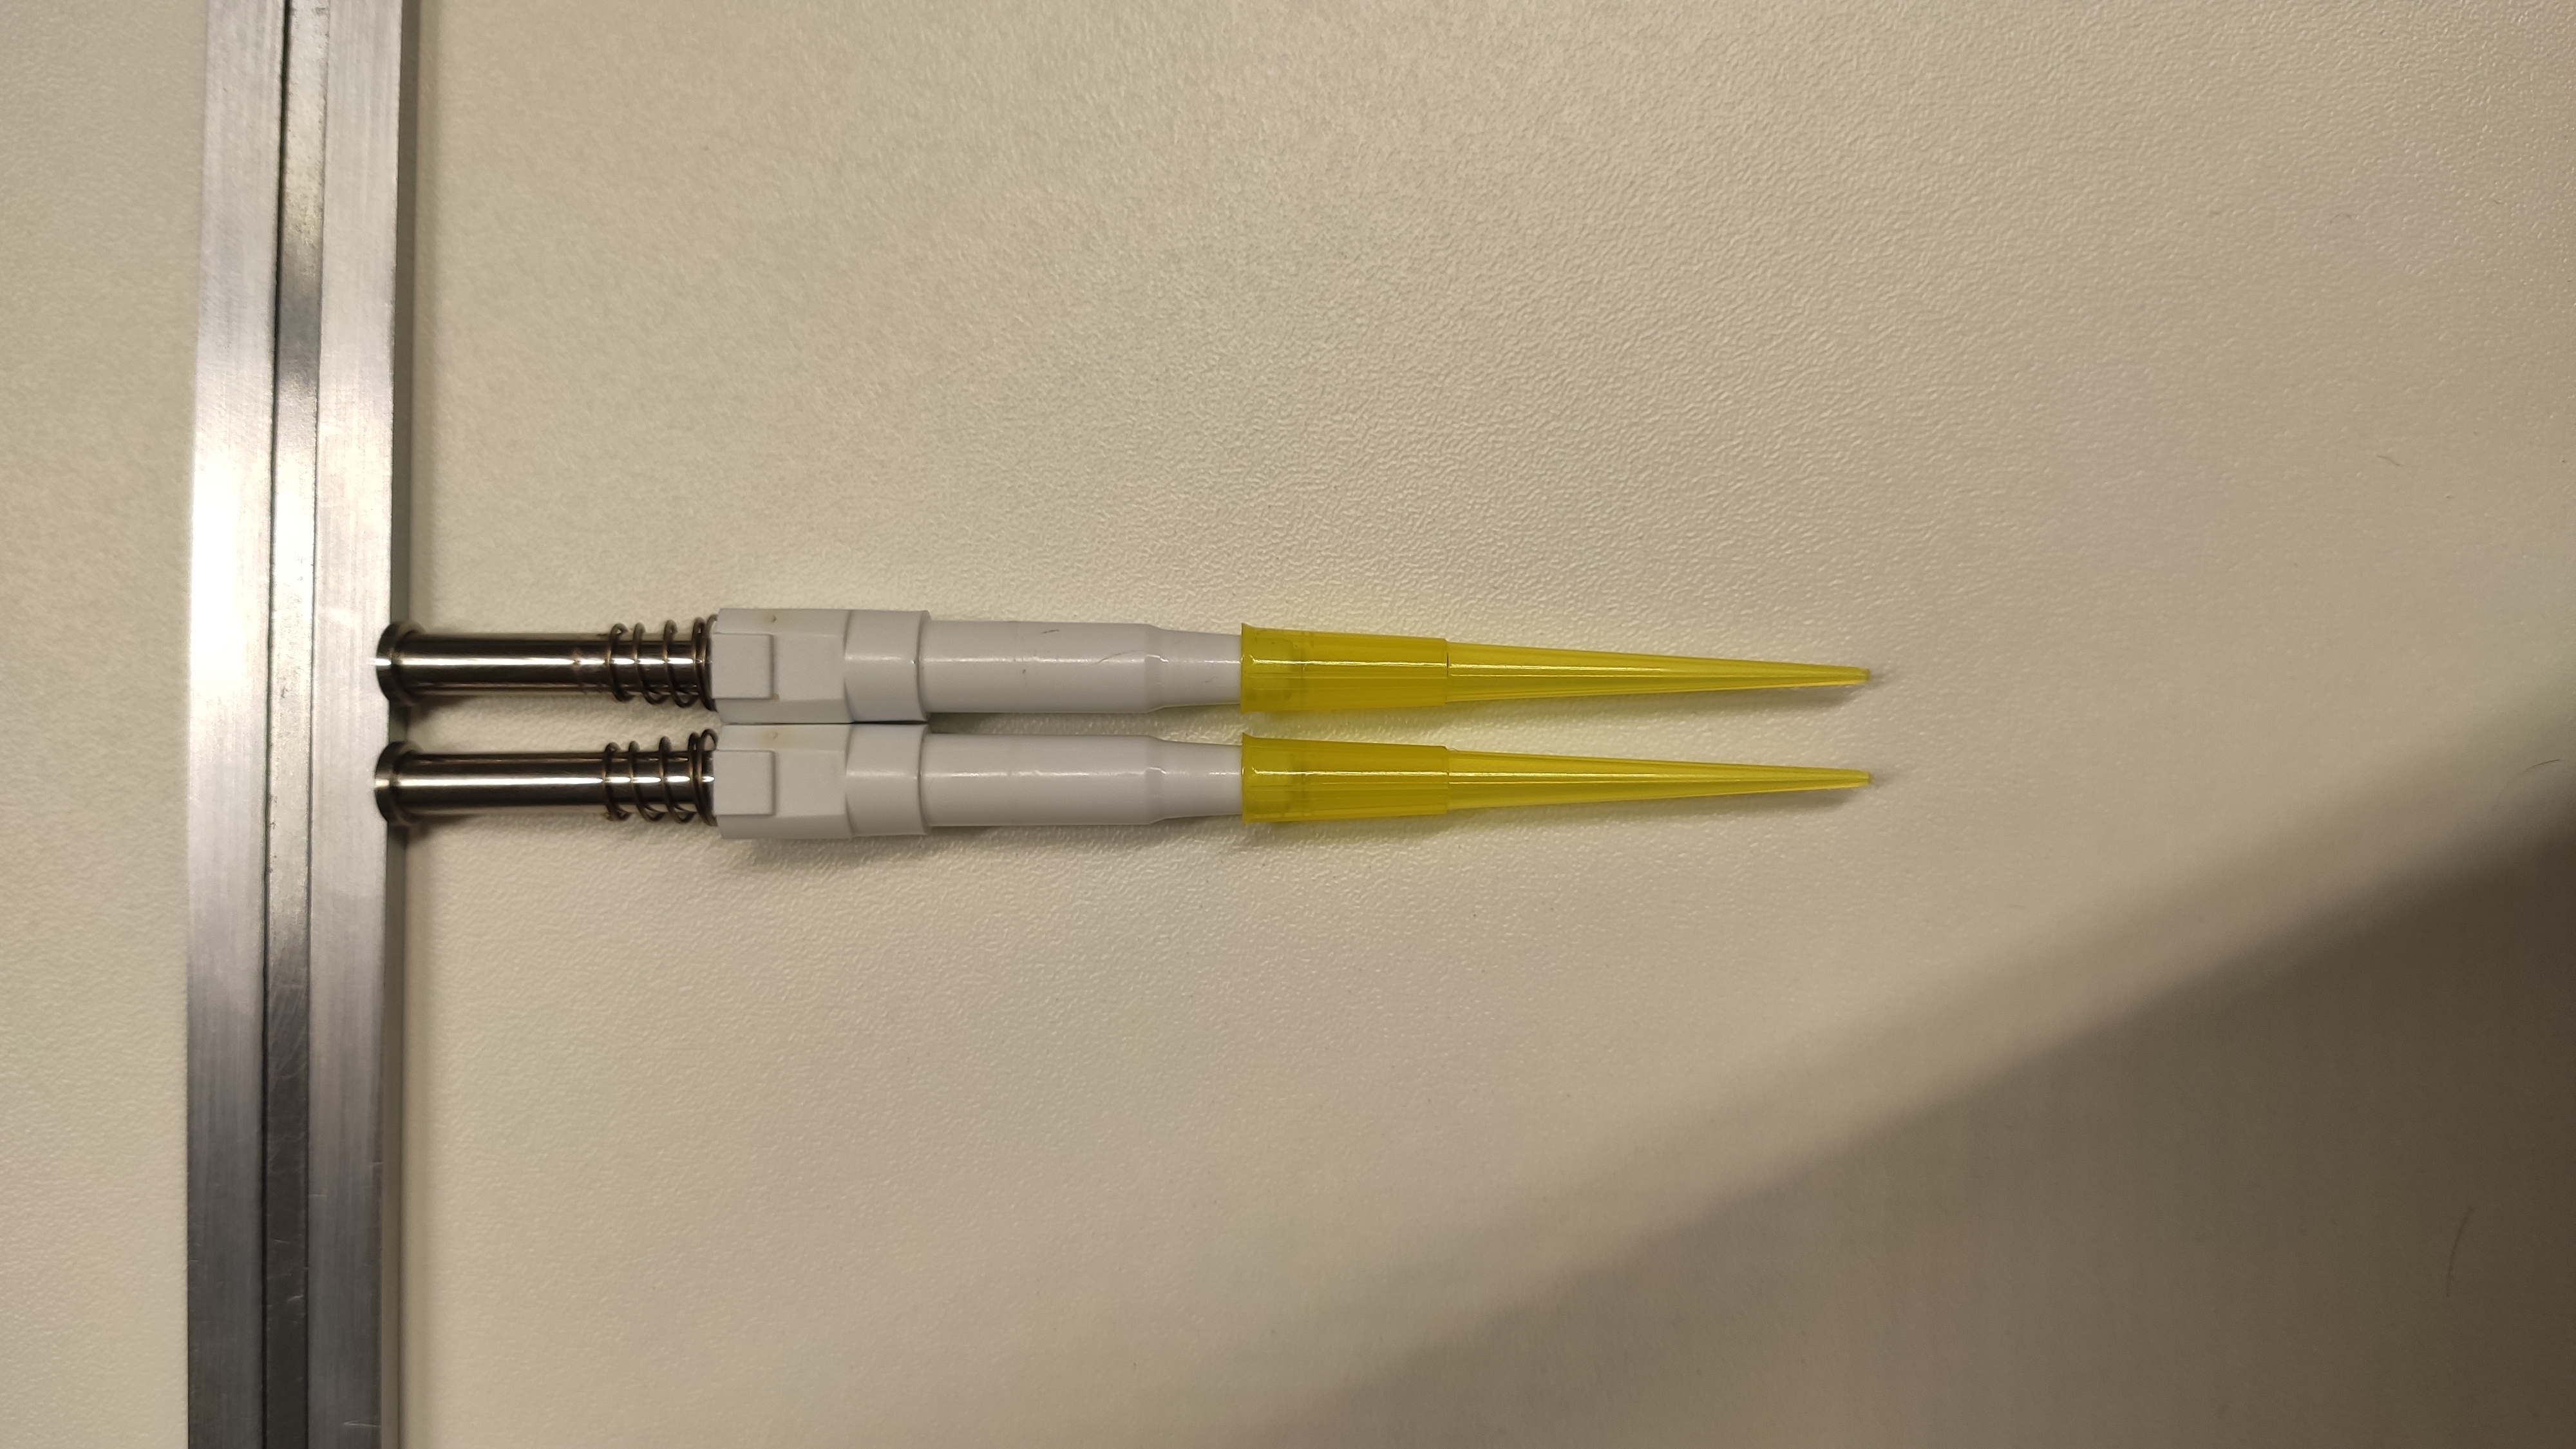
\includegraphics[width=0.7\linewidth,angle=270]{fotoConcept1Zuiger(1).jpg}
		\caption{Plaat aan de koppen van de zuigers omhoog}
	\end{subfigure}%
	\begin{subfigure}{.5\textwidth}
		\centering
		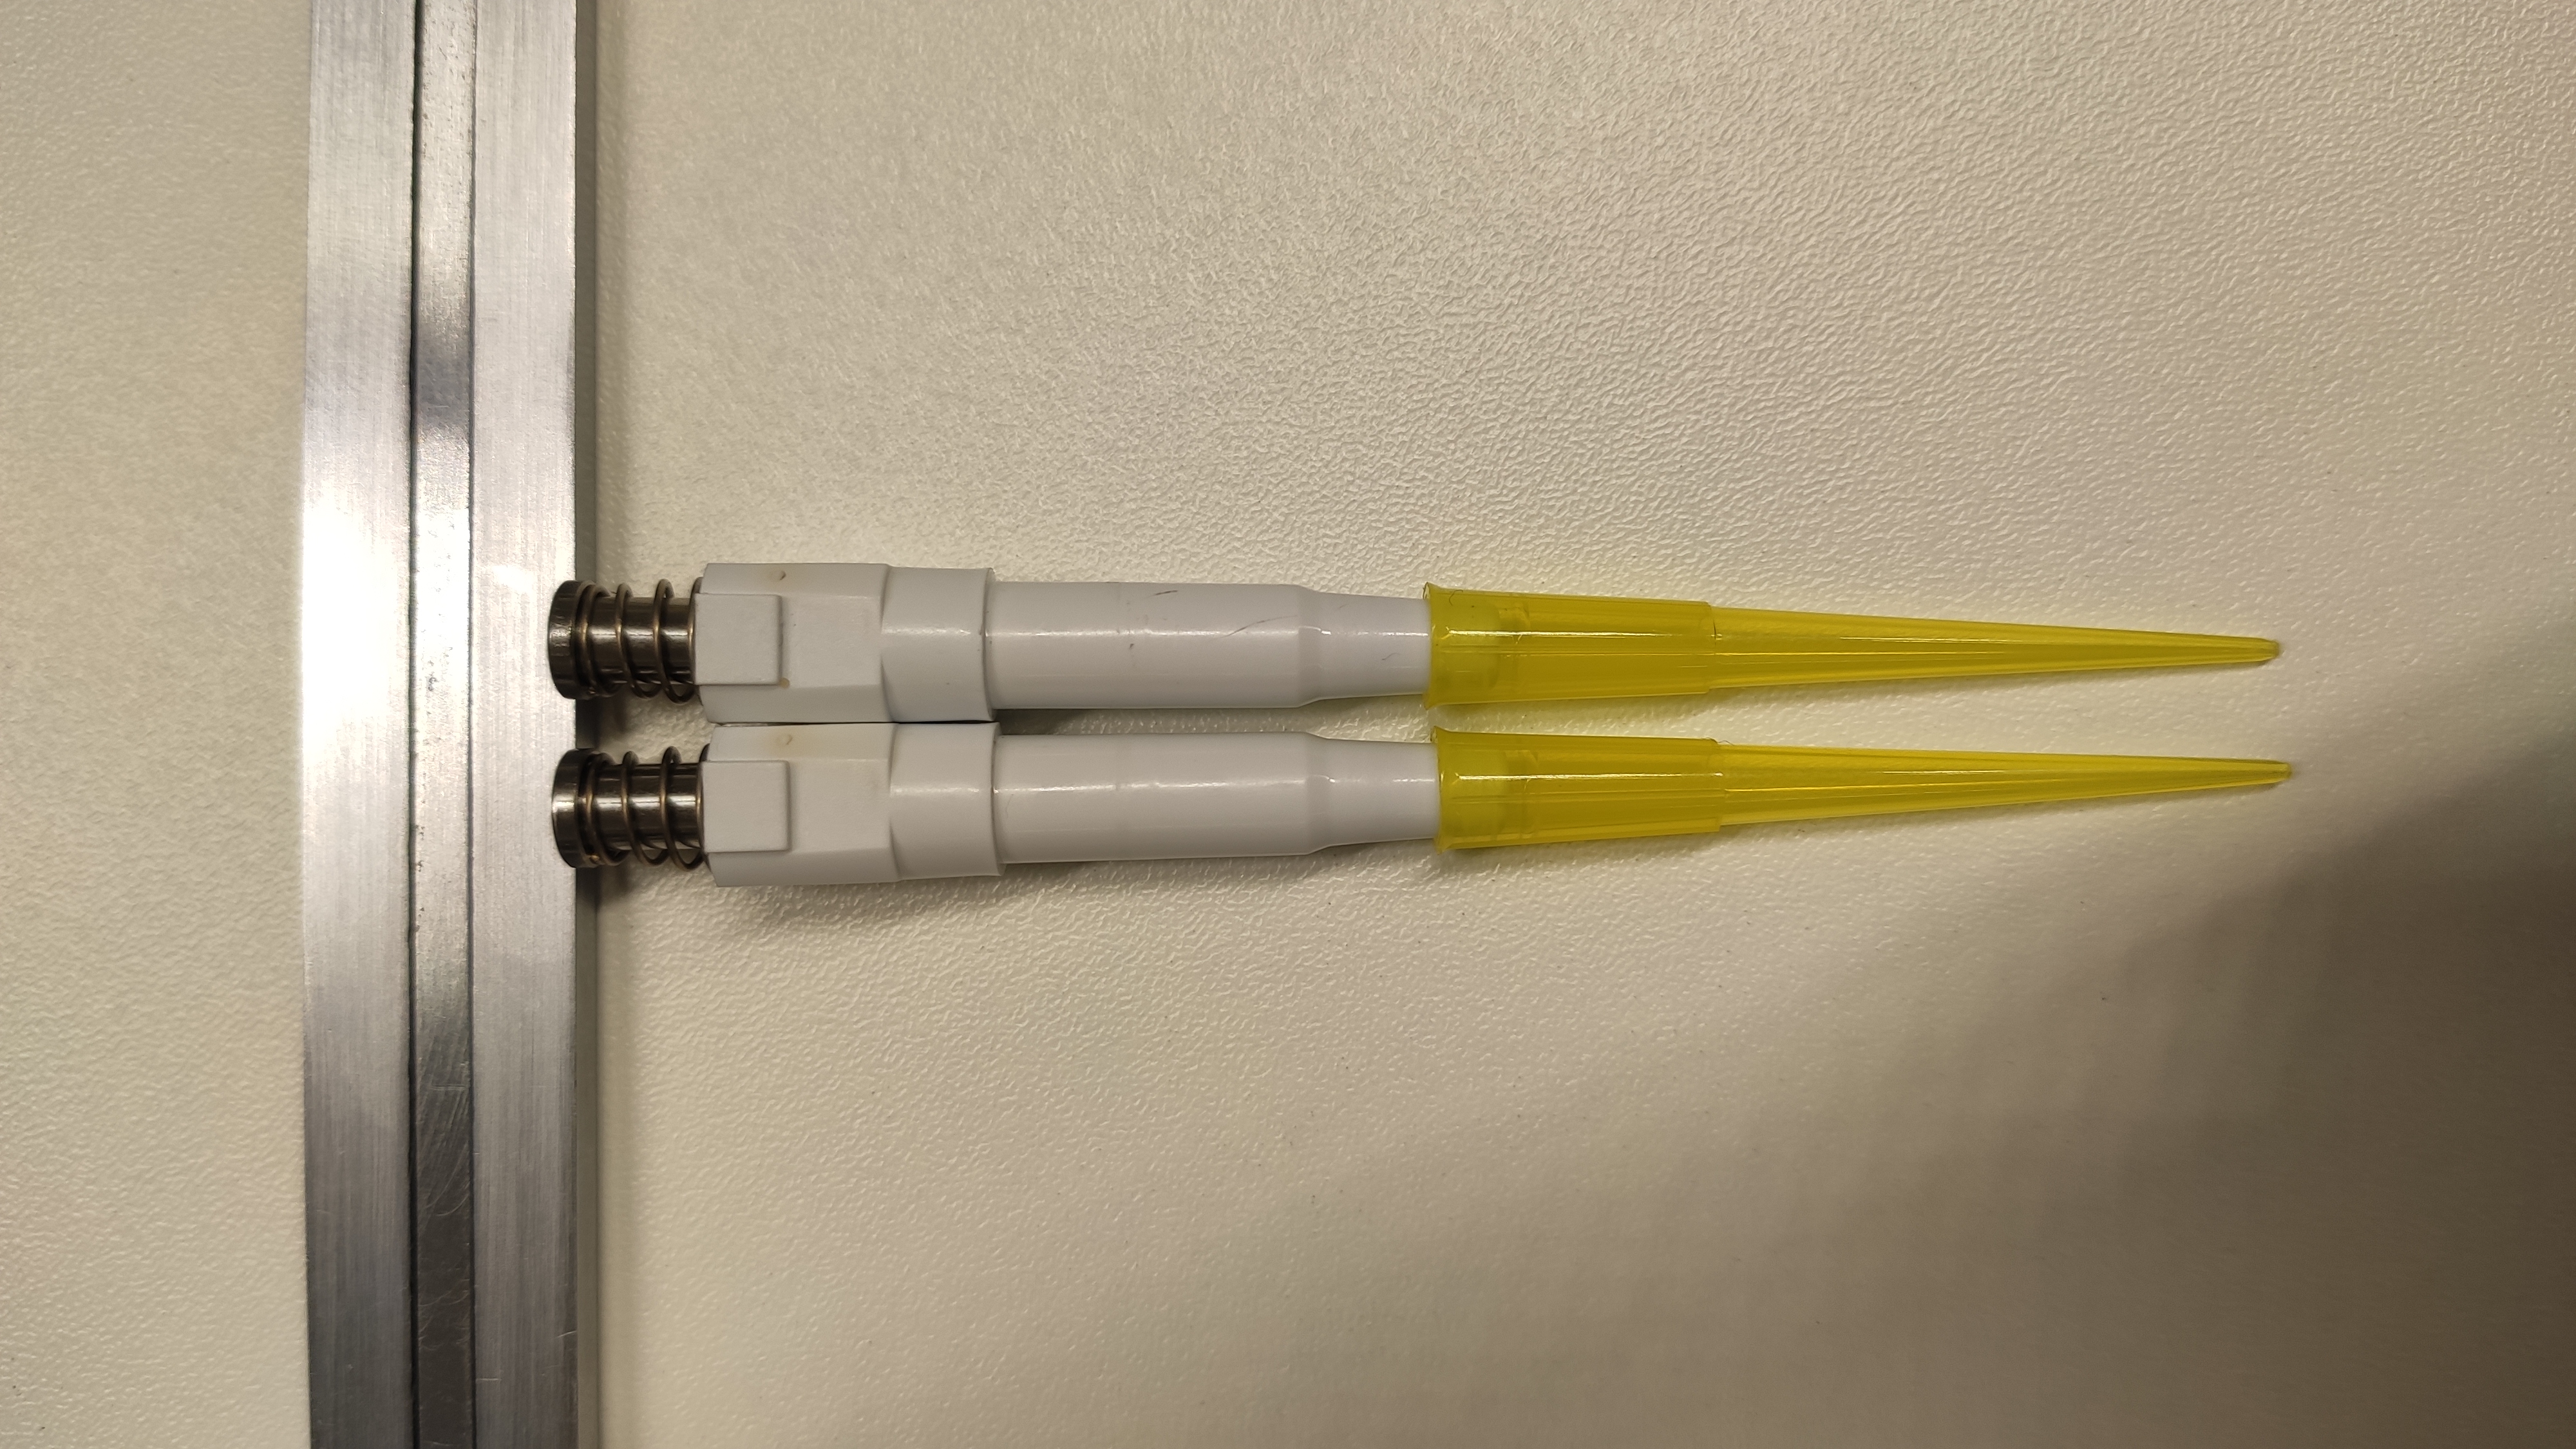
\includegraphics[width=0.7\linewidth,angle=270]{fotoConcept1Zuiger(2).jpg}
		\caption{Plaat aan de koppen van de zuigers omlaag}
	\end{subfigure}
	\label{fig: foto concept 1 zuiger}
\end{figure}

\subsection{Concept 2}
Het tweede concept is qua mechanisme om de \textit{wells} te vullen gelijkaardig, alleen worden hier minder cilinders en zuigers gebruikt. In Figuur \ref{fig: schets concept 2} staat een schets van het \textit{concept}. Er worden acht cilinders naast elkaar vastgemaakt aan een plaat, met opnieuw een afstand van 9 mm tussen de middelpunten van twee aanliggende cilinders. De zuigers die in de cilinders zitten, worden op analoge manier bevestigd als in \textit{concept} 1. In plaats van de \textit{wells} in de plaat in een keer te vullen, gebeurt dit nu in twaalf stappen. Telkens wanneer een rij van acht \textit{wells} gevuld is, schuift de \textit{microwell}-plaat naar rechts, weg van onder de cilinders, en beweegt het geheel met de zuigers en cilinders naar onder en weer naar boven om de cilinders opnieuw te vullen met vloeistof. Vervolgens schuift de \textit{microwell}-plaat opnieuw naar links onder de cilinders en wordt weer een rij van 8 \textit{microwells} gevuld.

\begin{figure}[h]
	\centering
	\includegraphics[width=0.8\textwidth]{fotoConcept2.jpg}
	\caption{Schets \textit{concept} 2}
	\label{fig: schets concept 2}
	
\end{figure} 

\subsection{Concept 3}
Het derde \textit{concept} is compleet verschillend van de eerste twee. In dit \textit{concept} (zie Figuren \ref{fig: CAD-model globaal} en \ref{fig: CAD-model ingezoomd}) wordt gewerkt met een pomp die de vloeistof uit het recipiënt oppompt en via een buizennetwerk verdeelt over acht pipetpunten waarvan de middelpunten zich opnieuw op een afstand van 9 mm van elkaar bevinden. De afstand die de vloeistof aflegt van de pomp tot aan de uitgang van de pipetpunt is voor elk van de acht kanalen gelijk, wat belangrijk is om in elke \textit{well} even veel vloeistof te hebben. De \textit{microwell}-plaat wordt vastgemaakt aan een aandrijfriem en motor en kan op die manier verplaatst worden. Telkens wanneer een rij van acht \textit{wells} gevuld is, stopt de pomp en verschuift de \textit{microwell}-plaat 9 mm naar links. Daarna vult de pomp opnieuw acht \textit{wells}. Dit proces wordt herhaald tot de twaalf rijen van acht \textit{wells} gevuld zijn. 

\begin{figure}[h]
	\centering
	\includegraphics[width=0.8\textwidth]{micdis1.jpg}
	\caption{CAD-model \textit{concept} 3}
	\label{fig: CAD-model globaal}
	
\end{figure} 

\begin{figure}[h]
	\centering
	\includegraphics[width=0.8\textwidth]{micdis2.jpg}
	\caption{CAD-model \textit{concept} 3}
	\label{fig: CAD-model ingezoomd}
	
\end{figure} 

\section{Selectie concept}
In deze sectie worden per ontwerp de voordelen opgesomd en wordt de uiteindelijke keuze van een van de drie \textit{concepts} toegelicht.

\subsection{Voordelen}

\paragraph{Concept 1}
\begin{itemize}
	\item Snelste optie, want alle 96 \textit{wells} in één keer gevuld
	\item Uiterst precies, want er wordt gewerkt met vooraf geijkte cilinders zodat elke 	\textit{well} exact even veel vloeistof krijgt
\end{itemize}

\paragraph{Concept 2}
\begin{itemize}
	\item Goedkoper dan \textit{concept} 1
	\item Uiterst precies, want er wordt gewerkt met vooraf geijkte cilinders zodat elke 	\textit{well} exact even veel vloeistof krijgt
\end{itemize}

\paragraph{Concept 3}
\begin{itemize}
	\item Sneller dan \textit{concept 2}, want geen verticale bewegingen nodig
	\item Goedkoopste optie
	\item Eenvoudiger te maken dan \textit{concept} 1 en 2, want geen bewegingen in twee dimensies nodig
\end{itemize}

\subsection{Selectie uiteindelijk ontwerp}
Uiteindelijk werd gekozen voor \textit{Concept} 3. De doorslaggevende factor was hierbij de kostprijs. In het eerste en tweede \textit{concept} kosten de gebruikte zuigers en cilinders per stuk evenveel als het voorziene budget voor de gehele machine.





\chapter*{Besluit}
Afsluitende tekst.

\end{document}
